%! program = pdflatex

%\documentclass[12pt,a4paper]{memoir} % for a long document
\documentclass[12pt,a4paper,article]{report} % for a short document


\title{The Euskadi neutrino program at the European Spallation Source: Executive Progress Report.}
\author{J.J. Gómez-Cadenas, F. Monrabal \\ Donostia International Physics Center}
\date{July 2021} % Delete this line to display the current date
\usepackage{tcolorbox}
\usepackage{amsmath}
\usepackage[official]{eurosym}
\usepackage{xcolor}
\usepackage{makecell}



%%%Adjusting space between paragraphs
\setlength{\parskip}{12pt}

%%%%Hyphenation
 \hyphenation{TEK-NI-KER}

%%% BEGIN DOCUMENT
\begin{document}

\maketitle
%\tableofcontents* % the asterisk means that the contents itself isn't put into the ToC
\begin{centering}
\section*{Introduction}
\end{centering}
%\section{}
%\subsection{}
The construction of the European Spallation Source (ESS), opens a window of opportunity for the study of fundamental neutrino properties, taking advantage of the coherent emission of neutrinos produced in the decay at rest of positive pions at the spallation source. 

Developing such important contribution to Fundamental Physics is the  main objective of the $\mathbf{CoESS}$ international collaboration. This consortium, coordinated by Ikerbasque Professor Juan José Gómez Cadenas, aims to apply three different technologies for making high-statistics measurements of coherent neutrino scattering at the ESS, in an initial effort scheduled to last until the end of 2025.

The development and construction of a high-pressure Xe Time Projection Chamber (the $\mathbf{XeESS}$ detector) is one of the most significant scientific and technological milestones of the whole collaboration. This activity will entirely take place at the Basque Country, and will be carried on by the group lead by Ikerbasque Research Fellow Francesc Monrabal at Donostia International Physics Center (DIPC). The XeESS project has been described in detail in the scientific report titled \emph{"The Euskadi neutrino program at the European Spallation Source ($\nu$ESS)"} issued on October 2020. 


\begin{tcolorbox}


\emph{As described in the aforementioned report, the development and construction of the $\mathbf{XeESS}$  detector will require a sustained focus of resources during 4 years (2020-2024), plus one additional year or commissioning and yet another year for acquisition of the relevant scientific data. The scheduled agenda is ambitious but definitely achievable if the project has access to the required resources.}


\end{tcolorbox}

In this report, we will summarise the progress so far, paying special attention to the state the budget and the  agenda of the project. We will also analyse the impact of the COVID-19 pandemic on the project. We will finally provide detail about the budget spent and forecast, both for the rest of current year and next year. 


\newpage
\section*{Progress of project so far}


These initial period of the project has evolved according to the planned schedule and budget. Most of the activities have been centred around:
\begin{itemize} 
\item recruiting and training of the technical team,
\item preparing a fully dedicated laboratory space at DIPC,
\item establishing and consolidating strategic collaborations with both  Research/Technology Centers and industrial actors within the Territory,
\item completing the design of the main parts of the $\mathbf{XeESS}$  detector, and identifying the most significant technical difficulties of the manufacturing and assembly process. 
\end{itemize}
We will now describe in details each one of these aspects.
\subsection*{Recruitment of the Technical Team}
The profiles and required skills and experience of the members of the team, as described in our October 2020 report, were very clear to us, and so far we have not identified any further need.

 The recruitment stage has been completed quite successfully despite the difficulties imposed by the COVID-19 pandemic. Currently, the technical team is formed by Eva Oblak (Mechanical Engineer, previously at CIC-nanoGUNE), Rubén González Moreno (Applied Physicist, previously CTO at Bihurcrystal SL), Helena Almazán Molina (Post-doc, previously at Max Planck Institute, Heidelberg ) and Jose Luís López Gómez (Technician, previously at Hurtado Rivas SL). 
 
 The only position for which we have not yet found a suitable candidate is that of Electronic Engineer, although there is still a need for incorporating such a profile within the project
 
\subsection*{Preparation of Laboratory Space}
The DIPC has freed space in one of its buildings at its headquarters in Donostia, where the laboratory will remain hosted for the duration of the project (or until a better space within the Ibaeta campus becomes available). Supply of parts and equipment and fabrication of the main infrastructure have been carried on during the first half of the year, and will be installed in the laboratory during the second half. The facility will become operational along the last term of the year.

The development of the  $\mathbf{XeESS}$ detector requires access to very specific facilities, with essential infrastructure for safe handling of (expensive) gases (Xenon), and assembly of large mechanical parts. This is not standard equipment and has been developed and built specifically for the project (see Figure \ref{gascircuit}). In what concerns development of the electronics, the required equipment (oscilloscopes, high-voltage power-sources, etc) is available commercially.  

\begin{figure}[htbp]
\begin{center}
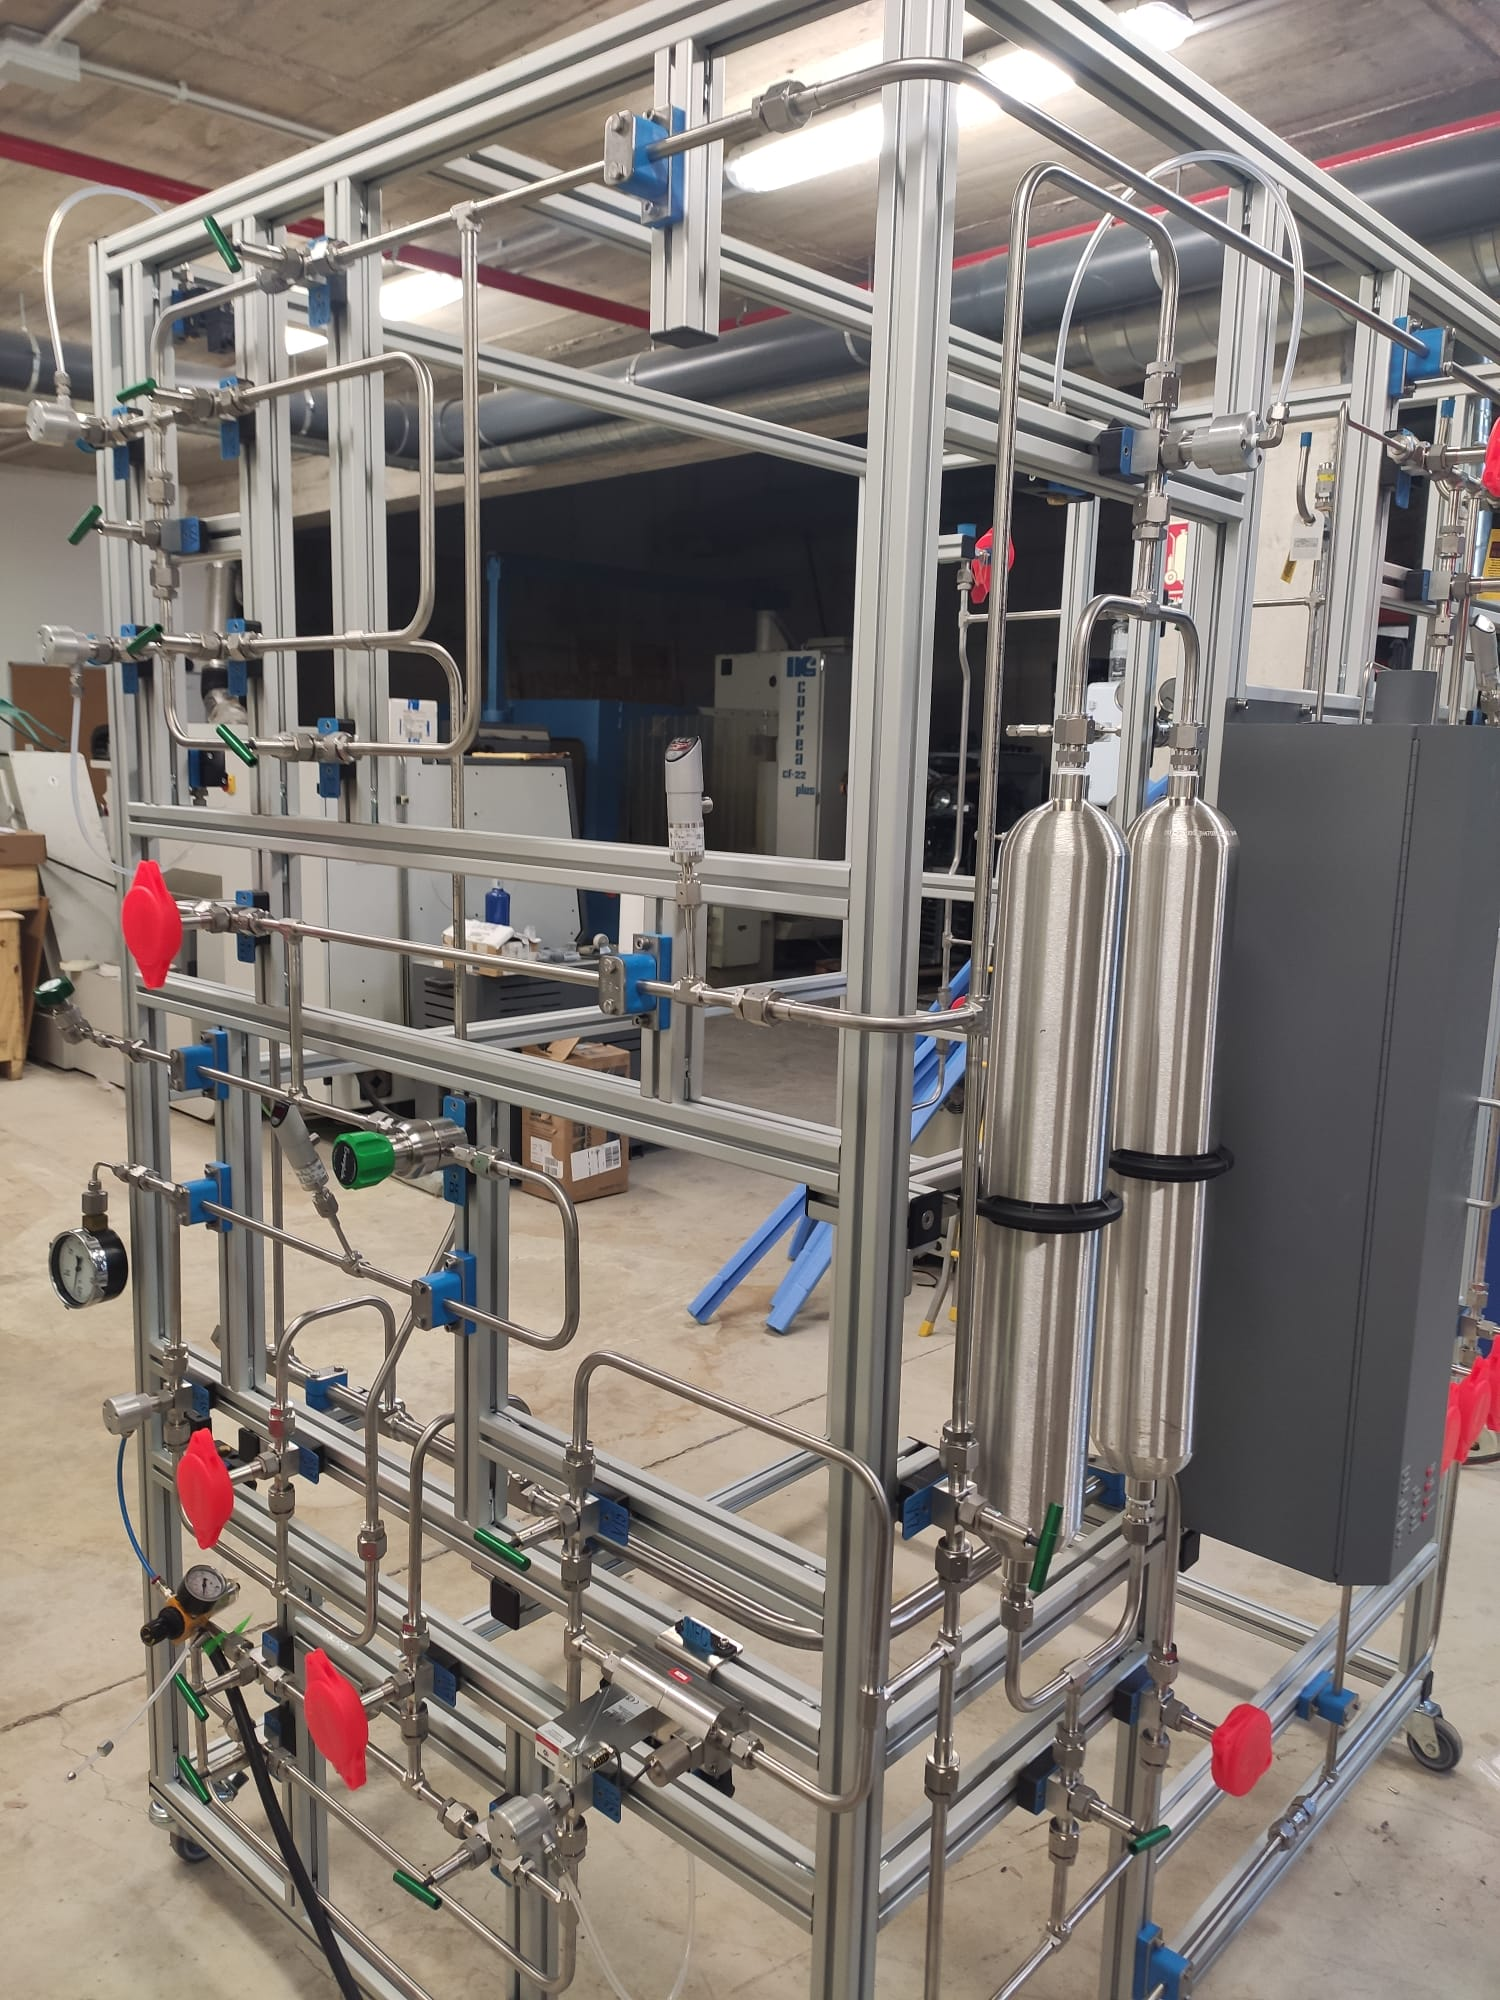
\includegraphics[width=6cm]{gascircuit}
\caption{\textbf{Gas handling system,} designed for safe fill and recovery of the Xe gas used in the $\mathbf{XeESS}$ detector. This infrastructure is installed in our laboratory space at DIPC.}
\label{gascircuit}
\end{center}
\end{figure}

\subsection*{Strategic Collaborations}
The possibility of interacting with the dense network of technological actors (both academic and industrial) present in the Basque Country is certainly a major asset of the project, because it gives us access to complementary skills and state-of-the-art manufacturing capacities which are essential for such complex objectives. During this first period, we have explored this network and identified the best partners.  A significant fraction of the 2021 budget will be invested in funding these ongoing collaborations. 

Several collaborations have already started and are producing the first results:
\begin{itemize}
\item \textbf{ TEKNIKER}, participates in the fabrication and characterisation of critical parts (large diameter high-voltage grids)  applying laser machining technologies. 
\item \textbf{ CEIT}, fabricates custom highly radiopure electronic components (high voltage resistors) using deposition and lithographic techniques in their clean room facilities. 
\item \textbf{AVS (Added Value Industrial Engineering Solutions, S.L.U.)} contributes to the development and manufactures a test bench for critical parts (test of high-voltage grids).
\end{itemize}

\begin{figure}[htbp]
\begin{center}
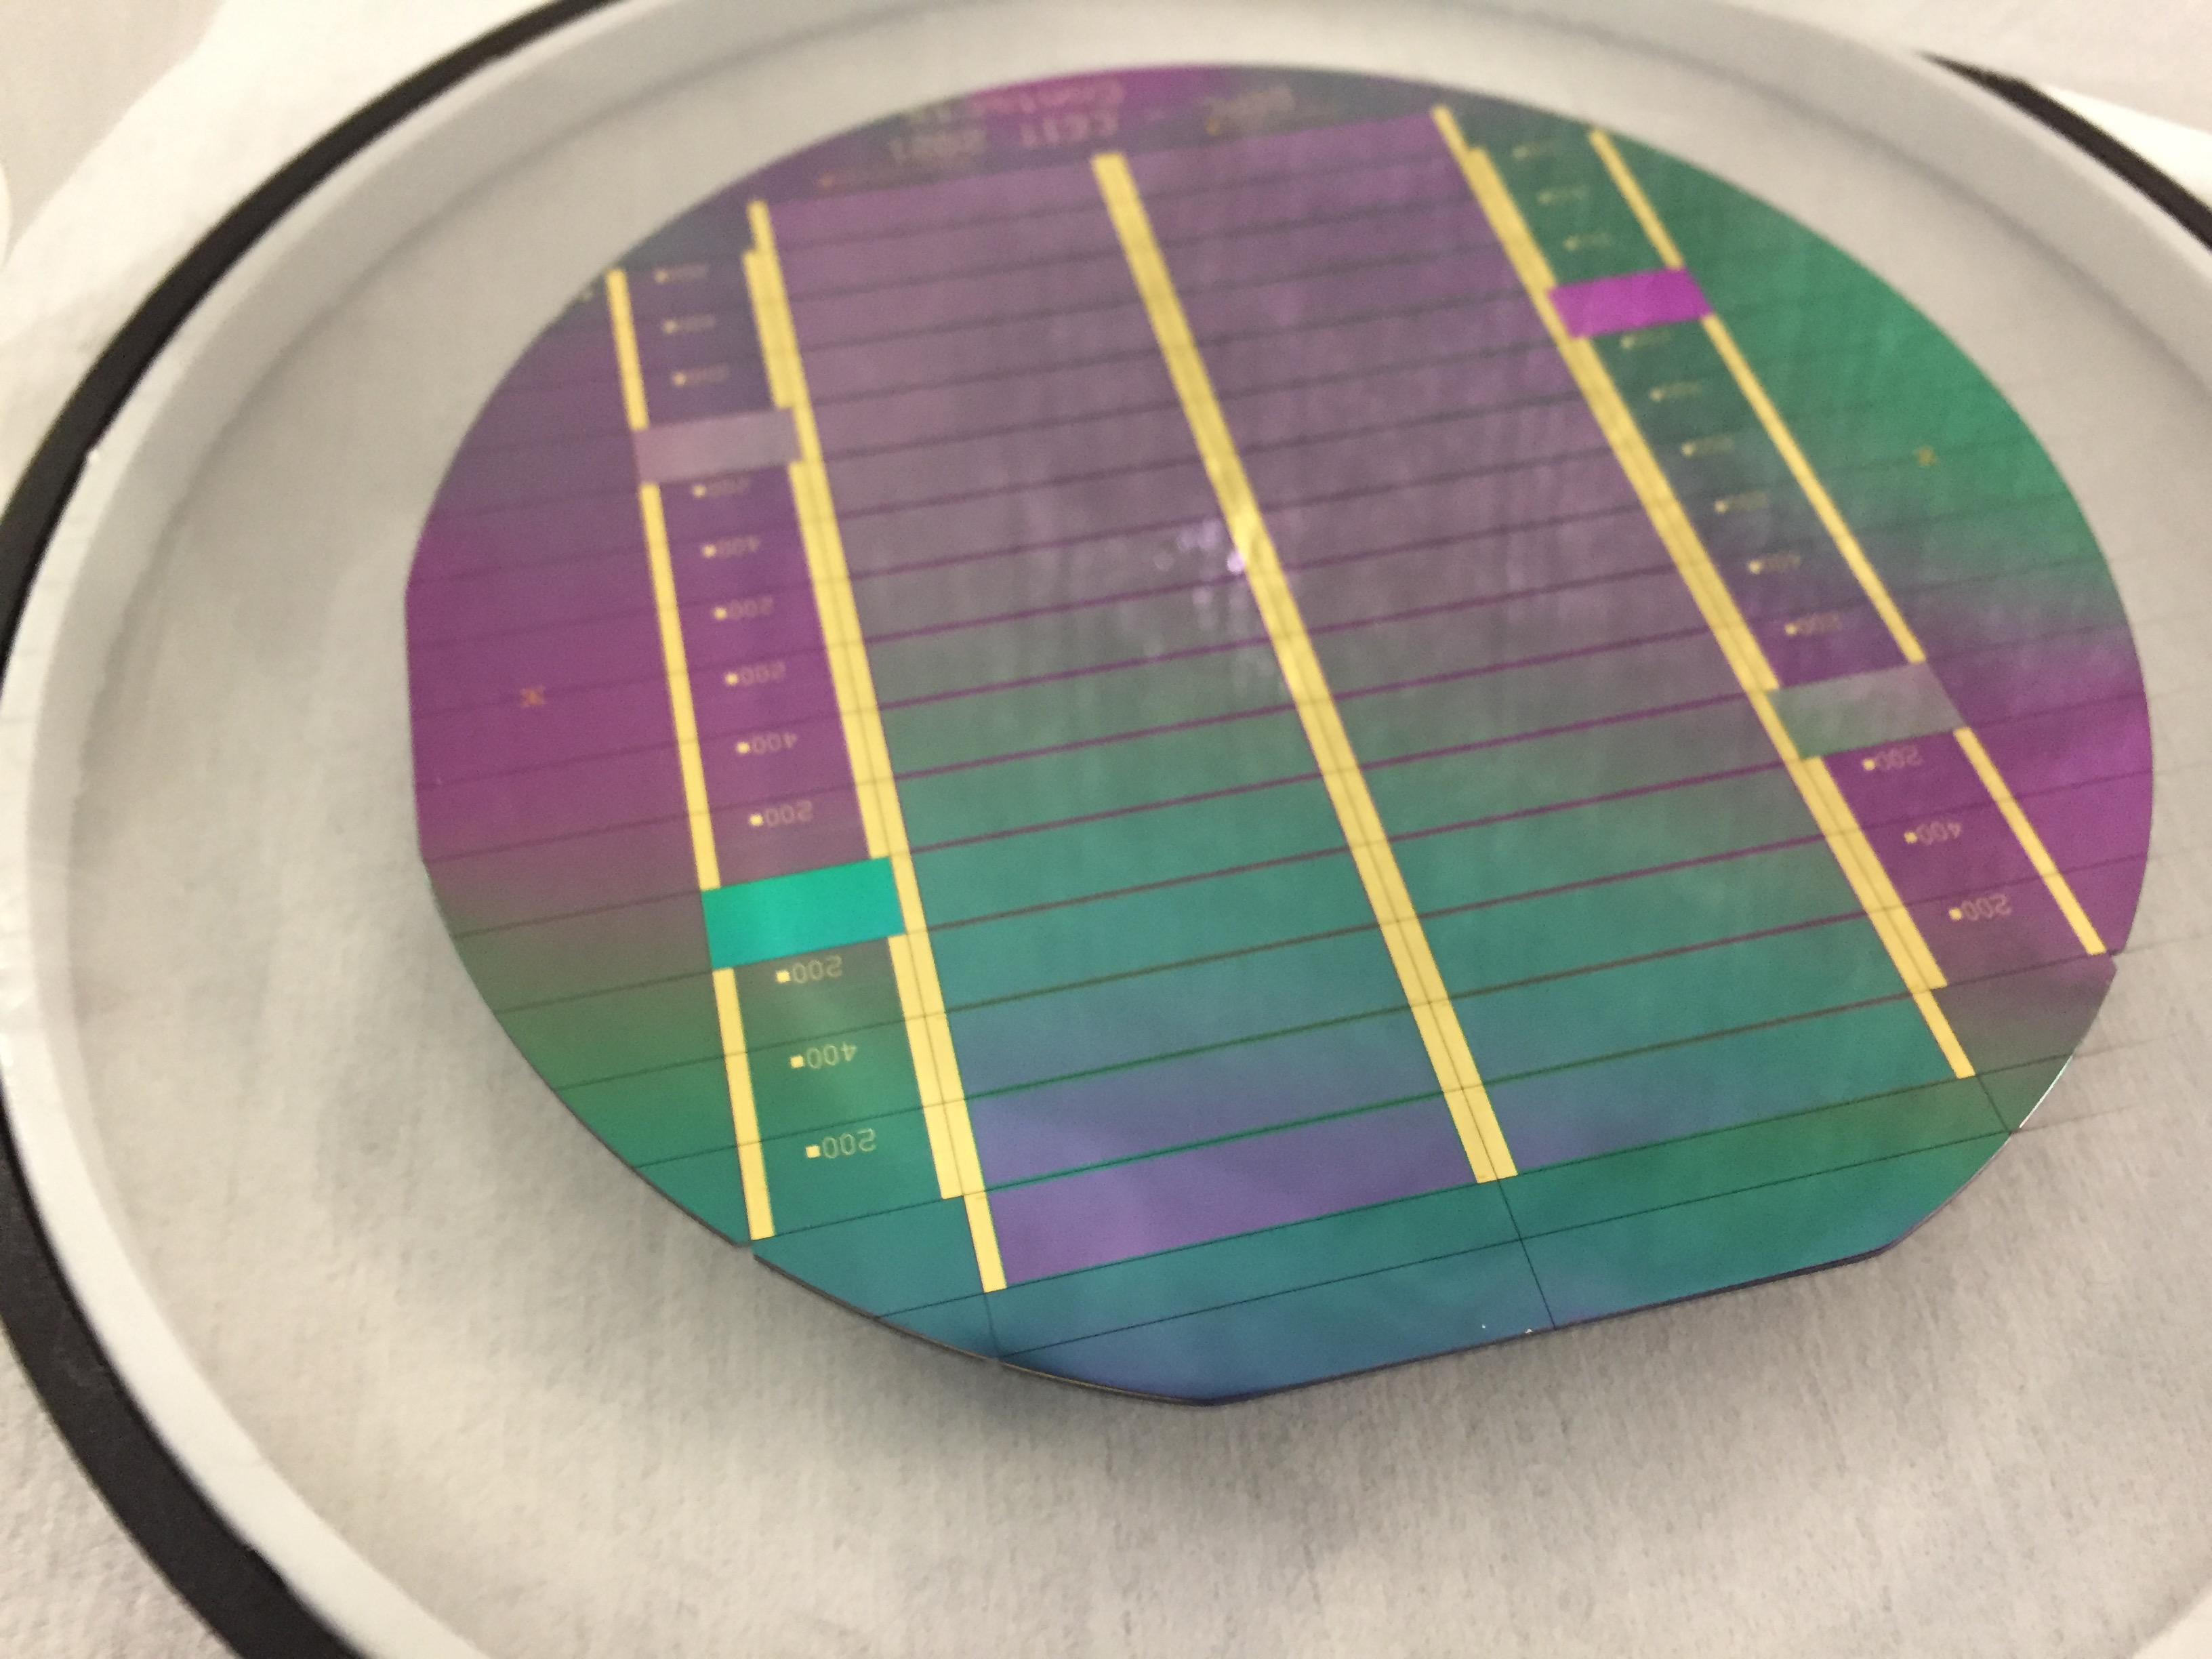
\includegraphics[width=6cm]{ceit} \hspace{1cm}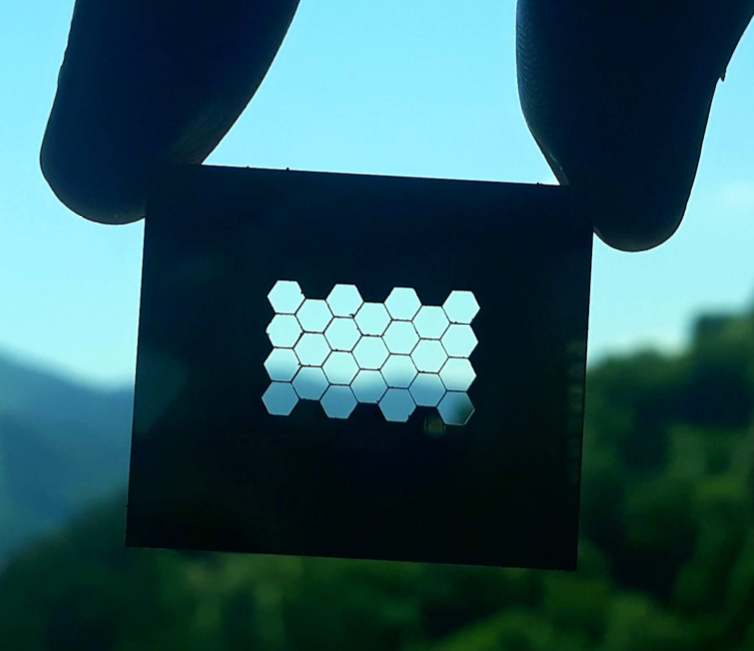
\includegraphics[width=6cm]{tekniker}
\includegraphics[width=6cm]{avs1} \hspace{1cm}\includegraphics[width=6cm]{avs2}
\caption{\textbf{Results from Strategic Collaborations}. High voltage electronic components (top left), developed with CEIT, laser manufacturing of critical parts (top right), developed with TEKNIKER, and test bench (bottom) being developed and constructed at AVS.}
\label{collaborations}
\end{center}
\end{figure}

We have also taken advantage of the network of long-term collaborators which have been contributing to the design of the NEXT experiment. This is the case of:
\begin{itemize}
\item \textbf{Laboratorio Subterraneo de Canfranc (LSC)} for the development of a manufacturing process for large parts made of radiopure Cu 
\item \textbf{Department of Nuclear Engineering of the Ben-Gurion University (Israel)} for the design of high-voltage grids. 
\end{itemize}

\subsection*{Design of the XeESS Detector}

The $\mathbf{XeESS}$ detector will be a high-pressure Xenon gas Time Projection Chamber (TCP), whose design takes advantage of the large experience accumulated during the development of the NEXT $0\nu\beta\beta$ experiment. 

The TCP concept is basically a pressurised vesseñ containing the Xe at high pressure. Interactions between the neutrinos produced at the spallation source and the Xe gas will  produce  events where a number of particles ($e^{-}$) and light resulting from scintillation. A large, high voltage, field applied along the chamber makes the particles drift, and arrays of sensors at the sides of the chamber allows to track and reconstruct the trajectory of these particles, which is characteristic and depends of the type of event.  During this first period, the efforts have been focused on the design of the main body of the vessel (shown in Figure \ref{chamber}). The design task will be finalised during the last term of the year, and this essential part of the system will be ready for fabrication along 2022.

\begin{figure}[htbp]
\begin{center}
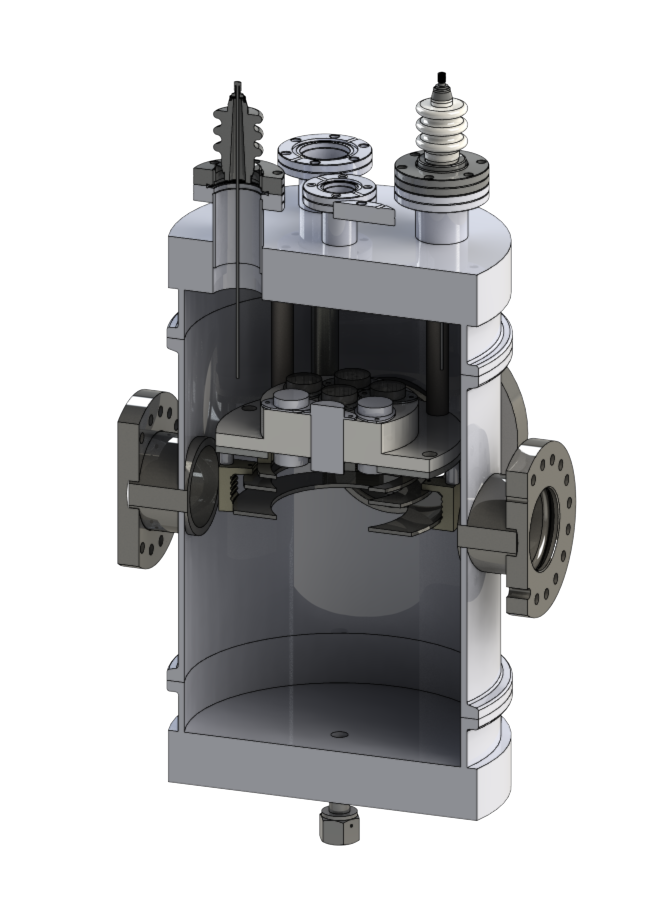
\includegraphics[width=6cm]{xeess1}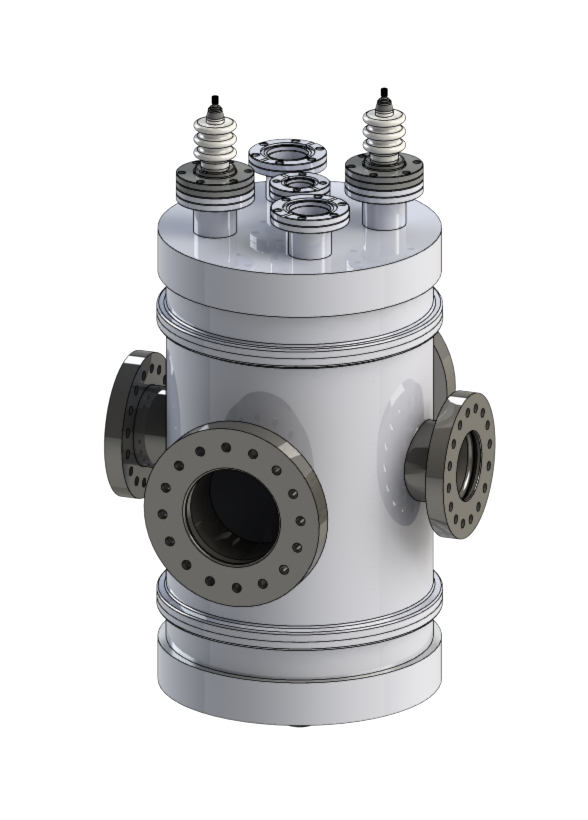
\includegraphics[width=6cm]{xeess2}
\caption{\textbf{Main vessel of the XeESS TCP detector.}}
\label{chamber}
\end{center}
\end{figure}

Another important aspect which has been studied in parallel is manufacturability. Some of the parts of the detector work under very severe conditions and their fabrication becomes a technical challenge, often beyond the capabilities of mainstream industrial actors. This is the case of some parts inside the detector which take the form of grids (see Figure \ref{grids}), and are designed to play the role of electrodes of a very large electrical field, while occupying a minimal fraction of surface and having as least mass as possible, in order to minimise noise and allow signals to pass through them with the leat interference. These parts work under very large amount of stress, caused by the electrical fields, that will cause bending of the structure. Surface finish of these elements is also important, as spikes and roughness will lead to a concentration of the electrical field, and cause electrical discharges that may damage parts of the detector. 

As mentioned previously, we have relied in some partners of the Basque Technological community for overcoming this important challenge. TEKNIKER is in charge of studying the feasibility of the manufacturing of the grids by means of different laser machining technologies. AVS will fabricate a test bench where the grids can be tested, both during the development stage and as part of the quality control when building the detector itself. 

\begin{figure}[ht]
\begin{center}
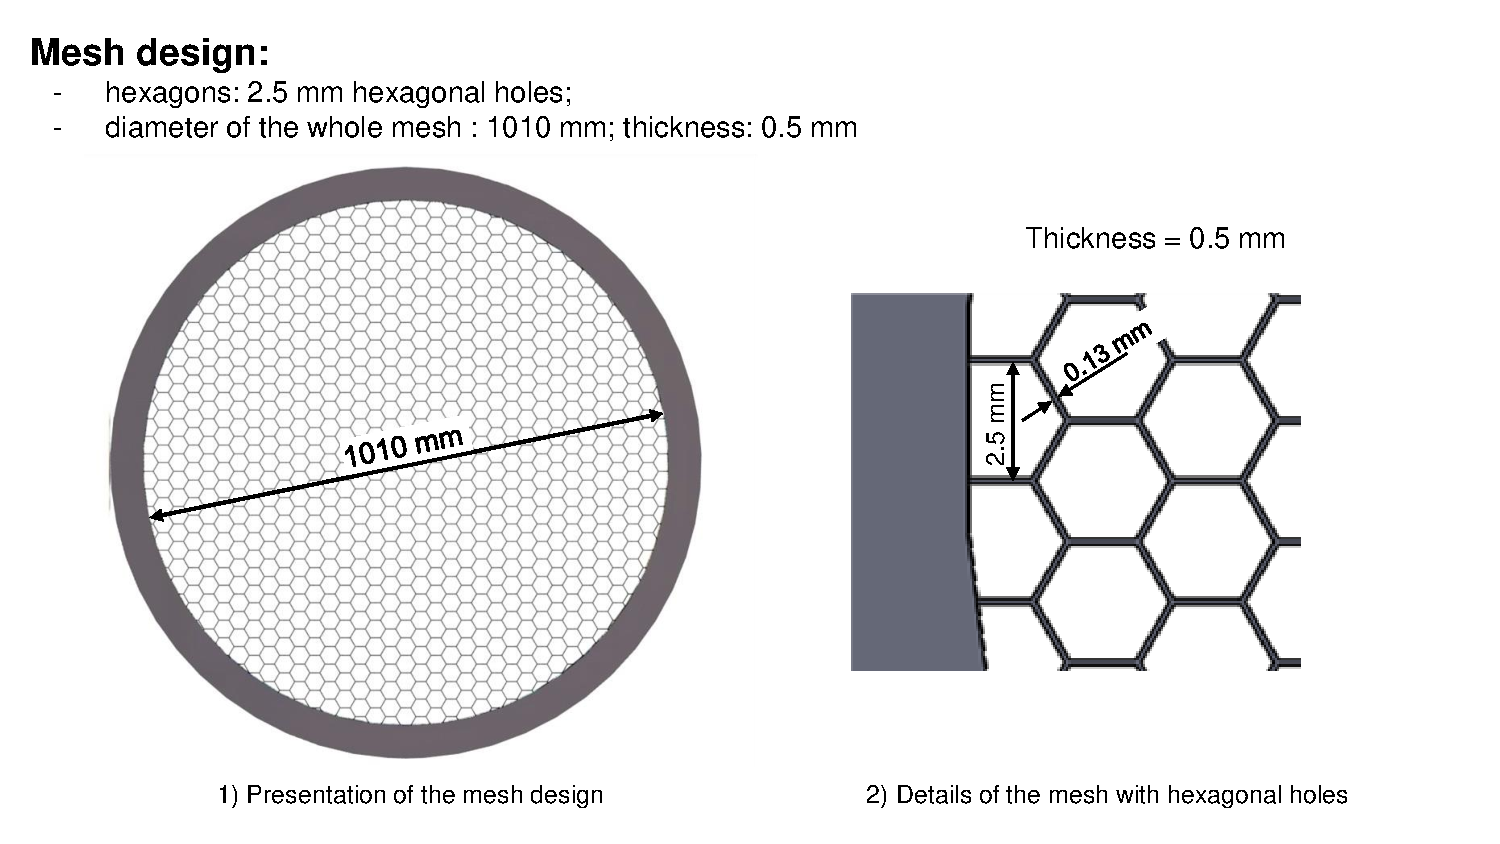
\includegraphics[width=14cm]{Grids}
\caption{\textbf{HighVoltage Grids,} will be placed inside the main chamber of the $\mathbf{XeESS}$ detector.}
\label{grids}
\end{center}
\end{figure}

\subsection*{Impact of COVID-19 Pandemic}

The unavoidable overlapping of this 2021 period  with the COVID-19 pandemic, has had a limited impact on the progress of the project. In particular, the strict mobility restrictions have made it impossible for us to visit the ESS site in Lund (Sweden), and forced us to keep the technical team under teleworking conditions during the second half of 2020 and most of the first half or 2021. The absence of visits to ESS at such an early stage of the project do not have any remarkable consequence, and the team has managed to coordinate their work using available teleworking tools (e-mail, videoconferencing, etc).

We have also experienced certain delays on the delivery of essential supplies, although the situation is recovering fast and we expect all mayor items for equipment of the laboratory space to be delivered and commissioned  by the end of the year 2021. As a matter precaution, the construction of the main elements of the $\mathbf{XeESS}$ detector (high-pressure chamber, etc) has been scheduled to take place along 2022, when we expect that the supply chains will have recovered normal operations pace. 

\subsection*{Budget Spent and Forecast}

We will first analyse the state of the budget for year 2021, detailed on table \ref{budget2021}. 

Initial estimated budget for Personnel Cost was  207.554,00 \euro{} , although  forecast for the period, taking into account salaries of the current team, is 178.432,00 \euro{}. As discussed previously, the difference mainly corresponds to uncovered Electronic Engineer post. The original forecasted sum will be fully required once the recruitment for this position is completed. 

Operations have been affected by the Covid-19 pandemic, and therefore only 8.389,38 \euro{} , out of an initial planned budget of 15.000,00 \euro{} are estimated to be used by the end of 2021. 

The budget section regarding equipment has been devoted mainly to the set up of the lab infrastructure, but also to the initiation of important strategic collaborations, as described already in the text. We have indeed devoted the remainders from other budget sections to reinforce these partnerships.

In what concerns the budget foreseen for year 2020, detailed in table \ref{budget2022}, it is worth outlining that we expect activity to reach full normality, with removal of the main restrictions regarding the control of the COVID-19 pandemic. We will therefore resume the original agenda which involve travelling to the ESS facilities, and therefore require planned budget for operations, as described in our original planning. 

Also Personnel and Equipment budgets remain as planned, as this investments are absolutely necessary for keeping the technical team and purchasing the main parts of the XeESS detector on time and without avoiding critical delays for the project.

\begin{table}[htp]
\caption{\large{\textbf{Budget Summary 2021}}}
\begin{center}
\begin{tabular}{p{0.25\linewidth}   r p{0.25\linewidth} r}

\textbf{Concept}&\makecell[l]{ \textbf{Spent/} \\ \textbf{Committed}}&\makecell[l]{  \textbf{Planned}}&\textbf{TOTAL}  \\  \hline\hline

{\footnotesize \emph{Mechanical Engineer }}&{\footnotesize \emph{57.805,12 \euro{} }}  & - &{\footnotesize \emph{57.805,12 \euro{} }}  \\ 
{\footnotesize \emph{Applied Physicist}}&{\footnotesize \emph{45.935,52 \euro{} }}  & - &{\footnotesize \emph{45.935,52 \ \euro{} }}  \\ \
{\footnotesize \emph{Post-Doc}}&{\footnotesize \emph{45.516,84 \euro{} }}  & - &{\footnotesize \emph{45.516,84 \euro{} }}  \\ 
{\footnotesize \emph{Technician }}&{\footnotesize \emph{29.172,12\euro{} }}  & - &{\footnotesize \emph{29.172,12 \euro{} }}  \\ \hline \\
\makecell[l] {\textbf{Personnel} \\  \textbf{Totals}}&\textbf{178.433,80 \euro{}}  & - &\textbf{178.433,80 \euro{} } \\  \\ \hline \hline 

{\footnotesize \emph{Computers \& IT}}&{\footnotesize \emph{1.149,49 \euro{} }}  & {\footnotesize \emph{1.853,00 \euro{} }} &{\footnotesize \emph{3.002,49 \euro{} }}  \\
{\footnotesize \emph{Lab. Supplies - valves}}&{\footnotesize \emph{1.259,12 \euro{} }}  & - &{\footnotesize \emph{1.259,12 \euro{} }}  \\
{\footnotesize \emph{Oscilloscope}}&{\footnotesize \emph{10.200,00 \euro{} }}  & - &{\footnotesize \emph{10.200,00 \euro{} }}  \\ 
{\footnotesize \emph{Xenon gas}}&{\footnotesize \emph{13,309,00 \euro{} }}  & - &{\footnotesize \emph{13,309.00 \euro{} }}  \\ 
{\footnotesize \emph{Col. TEKNIKER}}&{\footnotesize \emph{ 8.000,00 \euro{} }}  & - &{\footnotesize \emph{8,000.00 \euro{} }}  \\ 
{\footnotesize \emph{Col. CEIT}}&{\footnotesize \emph{ 1.814,00 \euro{} }}  & {\footnotesize \emph{ 2.810,00 \euro{} }}  &{\footnotesize \emph{4.624,00 \euro{} }}  \\ 
{\footnotesize \emph{Col. AVS}}&-  &{\footnotesize \emph{ 105.000,00 \euro{} }}&{\footnotesize \emph{105.000,00\euro{} }}  \\ 
{\footnotesize \emph{Col. LSC}}&-  &{\footnotesize \emph{ 30.000,00 \euro{} }}&{\footnotesize \emph{30.000,00\euro{} }}  \\ 
{\footnotesize \emph{Col. VGU}}&-  &{\footnotesize \emph{ 40.000,00 \euro{} }}&{\footnotesize \emph{40.000,00\euro{} }}  \\ 
{\footnotesize \emph{XeESS Electronics}}&-  &{\footnotesize \emph{ 45.000,00 \euro{} }}&{\footnotesize \emph{45.000,00\euro{} }}  \\ 
{\footnotesize \emph{Vacuum Pump}}&-  &{\footnotesize \emph{ 12.000,00 \euro{} }}&{\footnotesize \emph{12.000,00\euro{} }}  \\ 
{\footnotesize \emph{Gas Compressor}}&-  &{\footnotesize \emph{ 12.000,00 \euro{} }}&{\footnotesize \emph{12.000,00\euro{} }}  \\ 
{\footnotesize \emph{Res. Gas Analys.}}&-  &{\footnotesize \emph{ 10.000,00 \euro{} }}&{\footnotesize \emph{10.000,00\euro{} }}  \\ 
{\footnotesize \emph{Xe leak detector}}&-  &{\footnotesize \emph{ 40.000,00 \euro{} }}&{\footnotesize \emph{40.000,00\euro{} }}  \\ \hline \\



\makecell[l] {\textbf{Equipment} \\  \textbf{Totals}}& \textbf{35.731,61}  & \textbf{298.663,00 \euro{}} & \textbf{332.675,13 \euro{}}  \\  \\ \hline \hline 

{\footnotesize \emph{Travelling and Networking}}&{\footnotesize \emph{1889,38 \euro{} }}  &{\footnotesize \emph{6.500,00 \euro{} }}   &{\footnotesize \emph{8.389,38 \euro{} }}  \\ \hline \\

\makecell[l] {\textbf{Operations} \\  \textbf{Totals}}& \textbf{1.889,38 \euro{} }& \textbf{6.500,00 \euro{} }&\textbf{8.389,38 \euro{}}\\  \\ \hline \hline \\

\makecell[l] {\textbf{GRAND} \\  \textbf{TOTALS}}& \textbf{216.054,79} \euro{} & \textbf{305.163,00} \euro{} & \textbf{521.217,79 \euro{} }\\ 

\end{tabular}
\end{center}
\label{budget2021}
\end{table}%


			
\begin{table}[htp]
\caption{\large{\textbf{Budget Breakdown 2022}}}
\begin{center}
\begin{tabular}{r   r  r}


\textbf{Section}&\textbf{Concept}& \textbf{Amount}  \\ \hline \hline

&{\footnotesize \emph{Applied Physicist} }& {\footnotesize \emph{46.119,00 \euro{} }}\\ 
&{\footnotesize \emph{Post-Doc} }& {\footnotesize \emph{45.702,00 \euro{} }}\\ 
&{\footnotesize \emph{Mechanical Engineer} }& {\footnotesize \emph{42.432,00  \euro{} }}  \\
&{\footnotesize \emph{Electronics Engineer} }& {\footnotesize \emph{42.432,00 \euro{} }}\\
&{\footnotesize \emph{Technitian} }& {\footnotesize \emph{30.869,00 \euro{} }}\\ \hline \\

\makecell[r] {\textbf{Personnel} \\  \textbf{Totals}}&& \textbf{207.554,00 \euro{}}  \\ \\ \hline\hline 

&{\footnotesize \emph{XeESS1 Vessel (Collaboration)} }& {\footnotesize \emph{65.000,00 \euro{}}}\\ 
&{\footnotesize \emph{Vacuum System} }& {\footnotesize \emph{20.000,00 \euro{}}} \\ 
&{\footnotesize \emph{Evaporator (Collaboration)} }& {\footnotesize \emph{45.000,00  \euro{} }} \\
&{\footnotesize \emph{TPC  (Collaboration)} }& {\footnotesize \emph{20.000,00 \euro{}}} \\
&{\footnotesize \emph{High Voltage Feedthrough  (Collaboration)}} & {\footnotesize \emph{20.000,00 \euro{} }}\\ 
&{\footnotesize \emph{Emergency Gas Recovery System  (Collaboration)}} & {\footnotesize \emph{30.000,00 \euro{} }}\\ 
&{\footnotesize \emph{Photo-Multiplier Tubes}} & {\footnotesize \emph{40.000,00 \euro{}}} \\ 
&{\footnotesize \emph{Xenon gas}} & {\footnotesize \emph{52.446,00 \euro{} }}\\ \hline \\

\makecell[r] {\textbf{Equipment} \\  \textbf{Totals}}&& \textbf{292.446,00   \euro{}}  \\ \\ \hline\hline \\


&{\footnotesize \emph{Internal Travel \& Networking}} & {\footnotesize \emph{10.000,00 \euro{}}}\\ 
&{\footnotesize \emph{Travel to and Stays at ESS}} & {\footnotesize \emph{15.000,00 \euro{} }}\\ \hline \\
\makecell[r] {\textbf{Operations} \\  \textbf{Totals}}&& \textbf{25.000,00   \euro{}}  \\ \\ \hline\hline \\
\textbf{GRAND TOTAL}&& \textbf{525.000,00 \euro{}}  \
\end{tabular}
\end{center}
\label{budget2022}
\end{table}%			
			
			

\end{document}